\documentclass[oneside, a4paper, final, 14 pt]{extarticle}
\usepackage[utf8]{inputenc}
\usepackage[english,russian]{babel}
\usepackage{vmargin}
\usepackage{graphicx}
\setpapersize{A4}
\setmarginsrb{2cm}{1.5cm}{1cm}{1.5cm}{0pt}{0mm}{0pt}{13mm}
\usepackage{indentfirst}
\linespread{1.5}
\sloppy

\newenvironment{compactlist} {
  \begin{list}{{$\bullet$}} {
    \setlength\partopsep{0pt}
    \setlength\parskip{0pt}
    \setlength\parsep{0pt}
    \setlength\topsep{0pt}
    \setlength\itemsep{0pt}
  }
}{
  \end{list}
  \smallskip
}

\begin{document}

\begin{titlepage}
  \centerline{Московский государственный университет им.~М.В.Ломоносова}
  \centerline{Факультет Вычислительной математики и кибернетики}
  \smallskip
  \small
  \centerline{Кафедра Системного программирования}
  \centerline{\hfill\hrulefill\hrulefill\hfill}
  \vfill
  \vfill
  \vfill
  \Large
  \centerline{Введение в диплом}
  \Large
  \begin{centering}
  {\bf Автоматизация процесса создания пользовательского интерфейса к отнологическим базам знаний заданной предметной области.\\}
  \end{centering}
  \normalsize
  \vfill
  \vfill
  \vfill
  \vfill
  \begin{flushright}
  Научный руководитель:\\ зав.~отд., д.ф.-м.н Серебряков~В.А.\\
  \vfill
  Студент: Пушин~К.П.\\
  Группа~528\\
  \end{flushright}
  \vfill
  \vfill
  \vfill
  \centerline{Москва,~2013}
\end{titlepage}

\setcounter{page}{2}

\setcounter{tocdepth}{2}
\tableofcontents
\newpage

\section{Семантическая паутина}

\emph{Семантическая паутина} это движение, возглавляемое Консорциумом 
Всемирной паутины (W3C)~\cite{article:semweb}. Цель движения~--- создать единый способ совместного 
использования информации приложениями, людьми или организациями, то есть значительно упростить 
процесс обработки информации. Кроме того, паутина позволяет автоматически устанавливать новые связи 
между данными.

Стоит заметить, что семантическая паутина это не замена текущей системе, чаще использующей язык 
разметки гипертекста (HTML), а дополнение к этой системе.

Для реализации цели были разработаны и стандартизованы специальные инструменты, языки и форматы, 
позволяющие работать с данными из заданной предметной области. Рассмотрим подробнее некоторые 
технологии.

\textbf{Среда описания ресурса} \cite{rdf} (\emph{RDF, Resource Description Framework})~--- модель для 
представления данных, в особенности~--- метаданных. Среда предоставляет утверждения о ресурсах в 
пригодном для машинной обработки виде. Ресурсом может быть абсолютно любая сущность. Утверждение о 
ресурсе имеет вид "<субъект~-- предикат~-- объект"> и называется \emph{триплетом}. Для обозначения 
каждого элемента используются \emph{уникальные идентификаторы ресурса (URI)}. Множество всех 
утверждений образует ориентированный граф, в котором вершинами являются субъекты и объекты, а ребра 
помечены предикатами. RDF имеет несколько различных вариантов представлений. Самый популярный на 
сегодняшний день~--- \emph{RDF/XML}.

\textbf{Язык описания онтологий} \cite{owl} (\emph{OWL, Web Onthology Language})~--- язык для описания
веб-онтологий. Термин \emph{онтология}, взятый из философии, это раздел, описывающий формы бытия.
Веб-онтология это набор знаний об определенной предметной области. Она может включать в себя описание
классов, свойств, экземпляров классов и операций над ними. Кроме того, онтологии могут описывать,
как получить из данной онтологии некоторые логические следствия.

\textbf{Язык запросов SPARQL} \cite{sparql} (\emph{SPARQL Protocol and RDF Query Language})~--- язык
запросов к данным, представленным в модели RDF и протокол для передачи этих запросов и ответов к ним.
Предоставление SPARQL-точек доступа является рекомендацией Консорциума при публикации данных во
всемирной паутине.

\bigskip
\section{Связанные открытые данные}

\emph{Связанные открытые данные} \cite{lod} (LOD, Linked Open Data)~--- метод публикации структурированных 
данных в стандартных форматах семантической паутины, при котором все данные связываются с ранее 
опубликованными. 

Основные принципы LOD, сформулированные Тимом Бернерсом-Ли:
\begin{compactlist}
  \item Использование URI для идентификации сущностей;
  \item Использование HTTP URI для того, чтобы эти сущности могли использоваться человеком;
  \item При обращении по URI предоставлять информацию о сущности в одном из стандартизованных 
  форматов, например, RDF или SPARQL;
  \item При публикации данных в сети также публиковать ссылки на схожие данные (используя URI).
\end{compactlist}
\begin{figure}
  \centering
  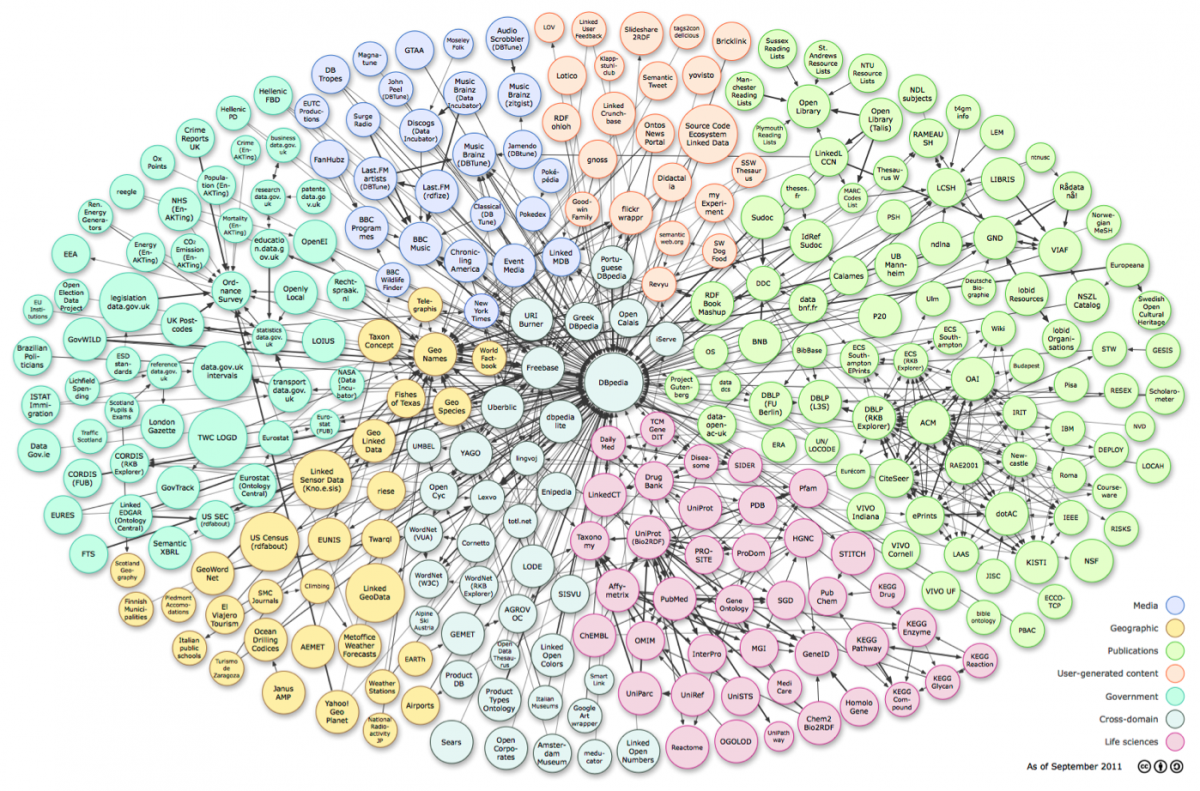
\includegraphics[width=0.8\textwidth]{cloud12.png}
  \caption{Диаграмма LOD}
  \label{lod:datasets}
\end{figure}

На~рис.~\ref{lod:datasets} показана диаграмма источников данных, опубликованных в LOD к 2012 году. Сейчас
можно сказать, что в развитии LOD наступила вторая фаза. В начале развития идеи (2006--2007 года)
основной задачей была публикация данных в сеть. Второй этап подразумевает улучшение "<экосистемы"> 
LOD. Основной проблемой всех данных является их избыточность и несвязность, поэтому появляются
различные приемы по автоматизации поиска уже опубликованных данных, относящихся к данной предметной
области и привязывания к ним своих данных.

\newpage
\section{Vocabulary of Interlinked Datasets}

\newpage
\section{Постановка задачи}

\newpage
\begin{thebibliography}{00}
  \bibitem{article:semweb}
  Berners-Lee~T., James~H., Lassila~O.
  \emph{The Semantic Web.}\\ Scientific American Magazine,  March 26, 2008.

  \bibitem{rdf}
  RDF\\
  \texttt{http://www.w3.org/TR/rdf-concepts/}

  \bibitem{owl}
  OWL\\
  \texttt{http://www.w3.org/TR/owl-semantics/}

  \bibitem{sparql}
  SPARQL\\
  \texttt{http://www.w3.org/TR/rdf-sparql-query/}

  \bibitem{lod}
  Heath~T., Bizer~C.
  \emph{Linked Data: Evolving the Web into a Global Data Space}\\ Synthesis Lectures on the Semantic Web: Theory and Technology, 2011.

  \bibitem{void}
  Keith~A., Cygainiak~R., Hausenblas~M., Zhao~J.
  \emph{On the Design and Usage of voiD, the ``Vocabulary Of Interlinked Datasets''}, LDOW, 2009.

\end{thebibliography}

\end{document}